\documentclass[12pt]{amsart}
\usepackage[pdftex,colorlinks,citecolor=blue,urlcolor=blue]{hyperref}
\usepackage{amssymb}
\usepackage{graphicx,color}
\usepackage{tikz}
\usepackage{amsmath}

\begin{document}

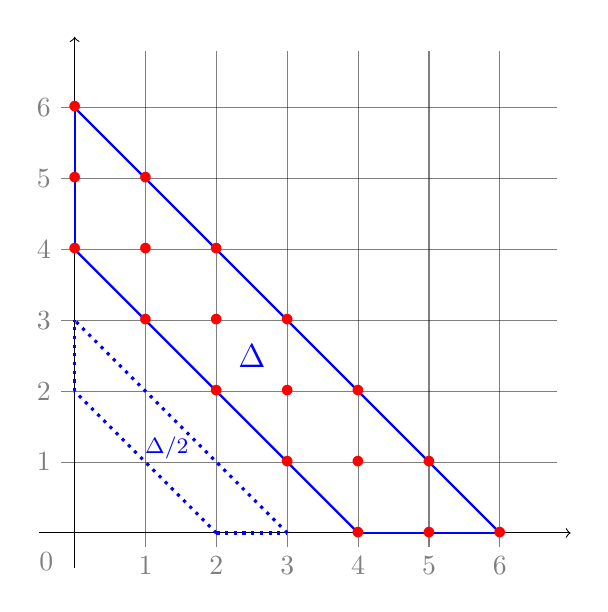
\begin{tikzpicture}[xscale=0.09,yscale=0.09,domain=0.125:220,samples=400]
  \node[opacity=0.5] at (-4,-4) {$0$};

  \draw[->] (-5,0) -- (70,0) node[below] {};
  \draw[->] (0,-5) -- (0,70) node[left] {};
  \foreach \i in {1,2,...,6} {
      \draw[opacity=0.5] (\i*10,68) -- (\i*10,-2) node[below] {$\i$};
  }
  \foreach \i in {1,2,...,6} {
      \draw[opacity=0.5] (68,\i*10) -- (-2,\i*10) node[left] {$\i$};
  }
  \draw[line width = 0.3mm, blue] (60,0) -- (0,60);
  \draw[line width = 0.3mm, blue] (40,0) -- (0,40);
  \draw[line width = 0.3mm, blue] (40,0) -- (60,0);
  \draw[line width = 0.3mm, blue] (0,40) -- (0,60);

  \node[blue] at (25,25) {{\large$\Delta$}};

  \draw[line width = 0.4mm, dotted, blue] (30,0) -- (0,30);
  \draw[line width = 0.4mm, dotted, blue] (20,0) -- (0,20);
  \draw[line width = 0.4mm, dotted, blue] (20,0) -- (30,0);
  \draw[line width = 0.4mm, dotted, blue] (0,20) -- (0,30);

  \node[blue] at (13,12) {{\footnotesize $\Delta/2$}};


  \draw[red] (40,0) node {$\bullet$};
  \draw[red] (50,0) node {$\bullet$};
  \draw[red] (60,0) node {$\bullet$};
  \draw[red] (30,10) node {$\bullet$};
  \draw[red] (40,10) node {$\bullet$};
  \draw[red] (50,10) node {$\bullet$};
  \draw[red] (20,20) node {$\bullet$};
  \draw[red] (30,20) node {$\bullet$};
  \draw[red] (40,20) node {$\bullet$};
  \draw[red] (10,30) node {$\bullet$};
  \draw[red] (20,30) node {$\bullet$};
  \draw[red] (30,30) node {$\bullet$};
  \draw[red] (0,40) node {$\bullet$};
  \draw[red] (10,40) node {$\bullet$};
  \draw[red] (20,40) node {$\bullet$};
  \draw[red] (0,50) node {$\bullet$};
  \draw[red] (10,50) node {$\bullet$};
  \draw[red] (0,60) node {$\bullet$};
\end{tikzpicture}

\end{document}